\documentclass[11pt]{article}
\usepackage[scaled]{helvet}
\usepackage[utf8]{inputenc}
\usepackage{graphicx}
\usepackage[font={small,it}]{caption}
\renewcommand\familydefault{\sfdefault} 
\renewcommand{\baselinestretch}{1.1} 
\usepackage[letterpaper, margin=1in]{geometry}

\title{Udacity Machine Learning Nanodegree\\ Project 4: Train a SmartCab to Drive}
\author{Wolfgang Steiner \\ \small{wolfgang.steiner@gmail.com}}
\date{August 2016}

\begin{document}


\maketitle

\section*{Task 1: Implement a Basic Driving Agent}
\textit{Observe what you see with the agent's behavior as it takes random actions. Does the smartcab eventually make it to the destination? Are there any other interesting observations to note?}\\

Given enough time, the agent will traverse the whole grid, following a random path and will reach the destination eventually. The rules of the game will not permit the smartcap to cross an intersection when the traffic lights are red or when another car has the right of way.
In case of an illegal action, the smartcap will stop for the respective time step and a penalty (= negative reward) will be assigned. The world is toroid, which means that agents can drive off one edge of the world and reappear on the opposite edge. 

\section*{Task 2: Inform the Driving Agent}
\textit{What states have you identified that are appropriate for modeling the smartcab and environment? Why do you believe each of these states to be appropriate for this problem?}\\

The following states are required for learning the agent's policy:
\begin{itemize}
    \item \textbf{next\_waypoint} \\
        The prime goal of the agent is to reach the destination in time. A rational agent will thus follow the direction that the planer has calculated for the current step.\\
        States: \textit{left}, \textit{right}, \textit{forward}.
    
    \item \textbf{light} \\
        The second requirement for the agent is to follow the traffic rules. The state of the traffic light at the current intersection is thus crucial to avoid penalties.\\
        States: \textit{red}, \textit{green}.

    \item \textbf{oncoming} \\
        This input reports whether another car is oncoming at the current intersection and the direction it will continue in. When the traffic light is green, the agent is not allowed to turn left if there is an oncoming
        car that goes either \textit{forward} or \textit{right}.\\
        States: \textit{none}, \textit{left}, \textit{right}, \textit{forward}.
        
    \item \textbf{left} \\
        This input reports whether another car is coming from the left at the current intersection and the direction it will continue in. When the traffic light is red, the agent is not allowed to take a right turn if there
        is a car coming from the left that goes \textit{forward}.\\
        States: \textit{none}, \textit{left}, \textit{right}, \textit{forward}.
    
\end{itemize}

The following inputs can safely be ignored by the agents:
\begin{itemize}
    \item \textbf{right} \\
        This input reports whether another car is coming from the right at the current intersection and the direction it will continue in. When the traffic light is green, this other car has to wait and can safely be ignored. When the traffic light is red, cars coming from the right also do not interfere with the legal right turn. 
        Because of this, this input can be ignored.\\
        States: \textit{none}, \textit{left}, \textit{right}, \textit{forward}.

    \item \textbf{deadline}\\
        The deadline reports how many steps the agent is allowed to take in the current trial before the deadline
        is reached and is decreased with every turn. Including the deadline does not make sense because the agent does not know its absolute position in the environment. Accordingly it does not know if a pending deadline will mean that it has to speed up (e.g. by breaking traffic rules) or that it is already close enough to not worry about it. Furthermore, including the deadline would increase the number of possible state by such a large amount that training the agent would not be possible anymore given the number of available trials/turns for training.\\
        States: Integer number $<\approx 70$.

\end{itemize}

\textit{How many states in total exist for the smartcab in this environment? Does this number seem reasonable given that the goal of Q-Learning is to learn and make informed decisions about each state? Why or why not?}\\

The number of states in this environment can be computed by multiplying the number of states for each input:
\begin{equation}
n_{states} = n_{next\_waypoint} * n_{light} * n_{oncoming} * n_{left}  = 3 * 2 * 4 =  96
\end{equation}
There are 90 training trials, with about 30 steps per trial (random, based on initial distance to destination). Assuming that at least two encounters are necessary to train each state/action pair, the number of states trainable in this environment would be $90 * 30 / 4 / 2 \approx 337$. Thus, the number of trials/steps is sufficient to reliably train the agent using this state space. Furthermore, the number of other cars in the simulation is low which means that the states for \textit{oncoming} and \textit{left} will be \textit{none} most of the time. This leaves $n_{states} = 6$ core states representing the basic behavior of the agent which will be easily learned given the number of available turns. Whether the agent will learn the remaining states involving other cars depends on the number of encounters during training which is pure chance. If not all of these additional states are encountered the result will be an agent that behaves well in the absence of other cars and could potentially take illegal actions when other traffic is present.

\section*{Task 3: Implement a Q-Learning Driving Agent}
\textit{What changes do you notice in the agent's behavior when compared to the basic driving agent when random actions were always taken? Why is this behavior occurring?}\\

After implementing the Q-learning algorithm, the agent will at first behave like before: it will move around the environment randomly. When more trials are completed, the behavior of the agent starts to change: it will start to follow the direction of the planer and move into the general direction of the destination. When even more trials have been completed, the agent will improve in following the directions of the planer and will also avoid penalties due to traffic rule violations.

This behavior can be explained like this:
\begin{itemize}
    \item At the beginning, the Q-table is empty and the agent explores the environment by choosing random actions.
    \item After every action, the $q$ value is calculated:
      \begin{equation}
          Q(s_t,a_t) :=  Q(s_t,a_t) + \alpha * (r_{t+1} + \gamma * \max\limits_a(Q(s_{t+1},a_{t+1})) - Q(s_t,a_t)),
      \end{equation} 
      with reward $r$, learning rate $\alpha$ and discount factor $\gamma$.
    \item The updated (or new) Q-value is stored in the q-table.
    \item When the agent finds the current state in the Q-table it will choose the action with the highest Q-value, otherwise a random action is taken.
    \item The more states have been recorded in the Q-table, the better the agent becomes in choosing the right action.
    \item In order to sustain exploration, a random action is taken, based on the parameter $\epsilon$.
    \item In later trials $\epsilon$ is diminished and the agent starts to rely on the best actions determined from the Q-table, thus following directions, avoiding 
    traffic rule violations and reaching the destination more and more reliably.
\end{itemize}

\section*{Task 4: Improve the Q-Learning Driving Agent}
\setcounter{section}{4} 
\subsection{Changes to the Q-learning Algorithm}

\subsubsection{Exploration vs. Exploitation}
In the first implementation of the agent, $\epsilon$ was initialized to 1.0 and then diminished by a factor of 0.975 for every trial. This results in a value of $\epsilon = 1.0 * 0.975^{89} \approx 0.105$ at the 90th trial. In this way the agent will explore new states early 
in the trials and will then gradually rely more on the Q-table for choosing the best action. On the other hand, it would be advantageous if the agent would spend as much time as possible exploring, as the there are a relatively high number of states. This can be achieved by letting the agent explore for the first 90 trials ($\epsilon = 1$), thus discovering as many states as possible. In the last 10 trials $\epsilon$ is set to zero, so that the agent can apply the learned policy without being disturbed by random actions.

\subsubsection{Learning Rate $\alpha$}
Usually the learning rate is initialized to some heuristic value and then diminished as the learning progresses. For highly stochastic environments a fixed value of $\alpha$ is also used. As I did not find an advantage of diminishing alpha during learning, I used the simpler implementation of a constant alpha. This also has the advantage that different values for $\alpha$ are easier to compare during grid search.

\subsubsection{Discounting Factor}
The discounting factor $\gamma$ determines how strongly future rewards are incorporated into the Q-value. In order to implement this, the action $a_{t-1}$, reward $r_{t-1}$ and state $s_{t-1}$ of the previous step are retained to update $Q(s_{t-1},a_{t-1})$ in time step $t$ while computing $\max\limits_a(Q(s_{t},a_{t}))$ for the current state $s_t$ and action $a_t$. For the case of $\gamma = 0$ an alternative code path is added which implements the much simpler
\begin{equation}
    Q(s_t,a_t) :=  Q(s_t,a_t) + \alpha * (r_{t+1} - Q(s_t,a_t)).
\end{equation}

Note that future awards are of limited utility in this environment as the next state the agent encounters is randomly generated by the environment. Increasing $\gamma$ will therefore tend to introduce more randomness into the Q-table (which might be advantageous in some cases).

\subsection{Metrics}
\begin{itemize}

\item \textbf{Success rate}\\
The number of successful trials is divided by the number of trials in a sample:
$$ \mathrm{success\_rate} = \frac{n_{success}}{n}. $$

\item \textbf{Penalty per step}\\
Training the agent to minimize the total penalty is crucial for a save driving experience. To derive a metric that is comparable 
across trials, the total penalty (= sum of negative rewards) is accumulated during the trial and divided by the number of steps taken 
by the agent during the trial:
$$ \mathrm{penalty\_per\_step} = - \frac{1}{n_{steps}}\sum\limits_{i, r_i < 0} r_i.$$

\item \textbf{Efficiency}\\
The agent should follow the directions given by the planer as accurately as possible in order to minimize the total distance traveled to the destination. To compare this performance between trials, the minimum number of steps from the starting position/heading is divided by the number of steps taken by the agent in the trial:
$$ \mathrm{efficiency} = \frac{n_{steps,min}}{n_{steps}}.$$
When the agent succeeds in finding the shortest route, the efficiency is equal to one. Note, that in some rare cases the efficiency can be greater as one. This happens when the agent starts at the edge of the world and has to make a u-turn as its first move. When the agents jumps to the opposite edge during this maneuver, the planer might then accidentally find a shorter route to the target. This case has not been considered when computing the minimal distance.
\end{itemize}

\subsection{Method}
One \textit{experiment} is defined as a set of 100 trials that are repeated 40 times. After set of 100 trials, the Q-table is cleared and the parameters $\gamma$, $\alpha$ and $\epsilon$ are reset to their starting values. Then, the mean values for the three metrics (success\_rate, penalty\_per\_step and efficiency) are computed.
In order to find the optimal values for $\gamma$ and $\alpha$, a grid search is performed by computing the mean values of the metrics while varying these two parameters. Code has been added to \textit{simulator.py} in order to compute the metrics during grid search.

\subsection{Results}
\textit{Report the different values for the parameters tuned in your basic implementation of Q-Learning. For which set of parameters does the agent perform best? How well does the final driving agent perform?}\\

The results of the grid search over $\gamma$ and $\alpha$ for the full state space are shown in Fig.~\ref{fig:full_state_space}. Performance is worst for high $\gamma$ and high $\alpha$. Here, future rewards, which are basically random, have a high influence on the learning algorithm. When this is combined with a high learning rate, the agent has a high randomness in its decisions. This can be seen in the relatively low success rate (0.94), high penalty per step (0.17) and especially in the low efficiency (0.47). The low efficiency means that the agent does not follow directions closely but instead meanders around before reaching the destination.

Success rate increases with reduced gamma and approaches 100\% for $\gamma <= 0.25$. Both penalty per step and efficiency clearly have the best values for $\gamma \le 0.125$ ($\le 0.001$ and $\ge 0.99$ respectively). The differences for $\gamma = 0.125$ and $\gamma = 0.0$ are small for all three metrics which suggests that the simpler implementation for $\gamma = 0.0$ could also be used. 

The influence of $\alpha$ is less pronounced than that of $\gamma$ but can be summarized as follows: For $\gamma \ge 0.25$ increasing $\gamma$ will degrade performance. For $\gamma \le 0.125$ the learning rate has nearly no influence on success rate and efficiency while tending to decrease penalty per step. 

\begin{figure}[ht]
    \centering
    \makebox[\textwidth][c]
    {
        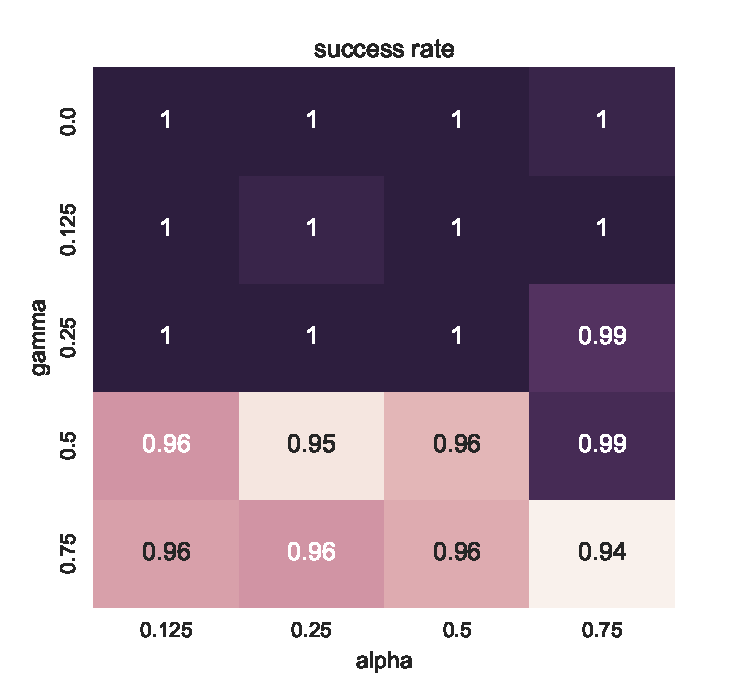
\includegraphics[width=0.4\linewidth]{fig/success}
        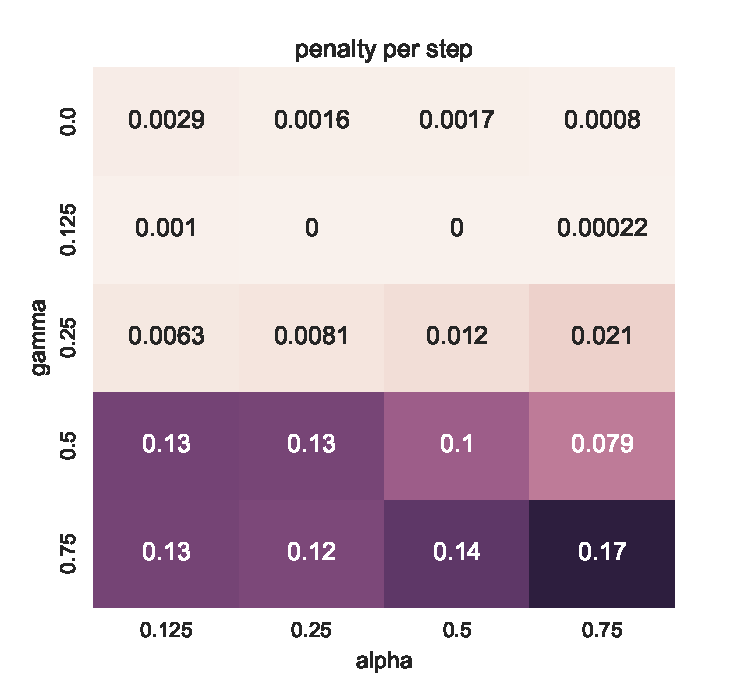
\includegraphics[width=0.4\linewidth]{fig/penalty}
        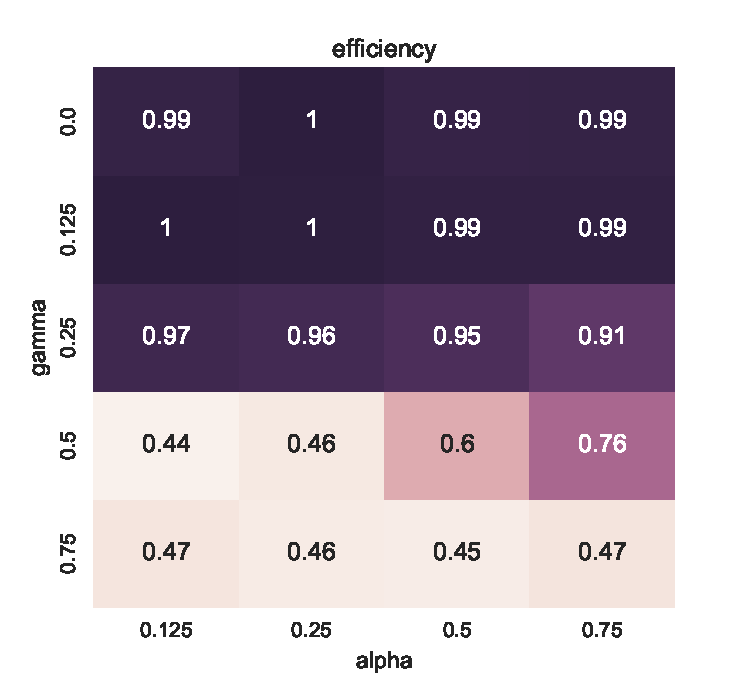
\includegraphics[width=0.4\linewidth]{fig/efficiency}
    }
    \caption{Results of the grid search over parameters $\gamma$ and $\alpha$ for the full state space.}
    \label{fig:full_state_space}
\end{figure}

Based on these result I have implemented the final version of the agent with $\gamma = 0.125$ and $\alpha~=~0.25$, where perfect scores where found during grid search. The first 90 trials are used for exploration ($\epsilon = 1$), while the last ten trials use the q-table ($\epsilon = 0$).

\subsection{Discussion}
\textit{Does your agent get close to finding an optimal policy, i.e. reach the destination in the minimum possible time, and not incur any penalties? How would you describe an optimal policy for this problem?}

I would argue that the agent is quite close to finding an optimal policy based on the scores of the three metrics defined. Success rate is nearly 100\%, penalties per step approach zero (0.00044 was reported during grid search) and the agent follows directions nearly perfectly (efficiency is found to be 1). In my opinion the optimal policy for the self driving cab could be described like this (in order of importance):
\begin{enumerate}
    \item Obey the traffic rules and do not endanger passengers and other road users.
    \item Follow directions of the planer as closely as possible.
    \item Reach the destination on time (follows from 1. and 2., if at all possible).
\end{enumerate}

\end{document}
